\section{Zigbee}

Zigbee jest standardem transmisji bezprzewodowej zapewniający niskokosztową platformą
możliwą do zastosowania w elektronice użytkowej, automatyce domowej, wszelkiego rodzaju sensorach
(w~szczególności przemysłowych i~medycznych) jak również grach i~zabawkach.
Pierwsza specyfikacja opublikowana została w grudniu 2004 roku będąc ciągle aktualizowana,
z najnowszą jej wersją będącą datowaną na marzec 2017 roku~\cite{zigbee_alliance_zigbee_2017}.

\lipsum[1-9]
\section{OpenThread}
\lipsum[1-10]

\section{Bluetooth Low Energy}
\lipsum[1-10]

\section{Porównanie przedstawionych standardów} % jako podroździał
% historia jako delikatny wstęp
\url{https://www.silabs.com/documents/public/application-notes/an1142-mesh-network-performance-comparison.pdf}
\url{https://www.silabs.com/wireless/matter}
\lipsum[1-15]


% 1. Krótki rys historyczny standardu
% 2. Opis stosu + jakiś obrazek
% 2.1. Częstotliwości na których pracuej standard
% 3. Topologia, rodzaje węzłów

\section{Teoretyczne podstawy opisywanych badań}
\section{Teoretyczne podstawy zaprojektowanych eksperymentów}

Celem tego podrozdziału jest zapewnienie minimalnego, teoretycznego wstępu
wymaganego do przeprowadzenia właściwych badań. Poniższe punkty
prezentują definicje, wzory i symulacje. Zawarte zostaną również
hipotezy badawcze, które w~praktycznej dalszej części pracy
zostaną empirycznie zweryfikowane.

\subsubsection{Badanie zużycia energii}
Energooszczędność urządzeń elektronicznych ma szczególne znaczenie w~przypadku produktów
zasilanymi ogniwami. Celem optymalizacyjnym jest wydłużenie czasu użytkowania na pojedynczym
ładowaniu bądź do kolejnej wymiany baterii.

Przed przystąpieniem do fizycznego eksperymentu, wykonano przykładową symulację z~użyciem
oprogramowania firmy ST, będącej producentem wybranej platformy opisanej w~kolejnym rozdziale.
\textit{STM32CubeMX} będący zintegrowanym środowiskiem programistycznym zapewnia moduł
o~nazwie \textit{PCC}~\cite{noauthor_um1718_2022}. Umożliwia on symulowanie zużycia energii 
przez układ zgodnie ze zgrubnymi szacunkami inżyniera.

\begin{figure}[!ht]
	\centering 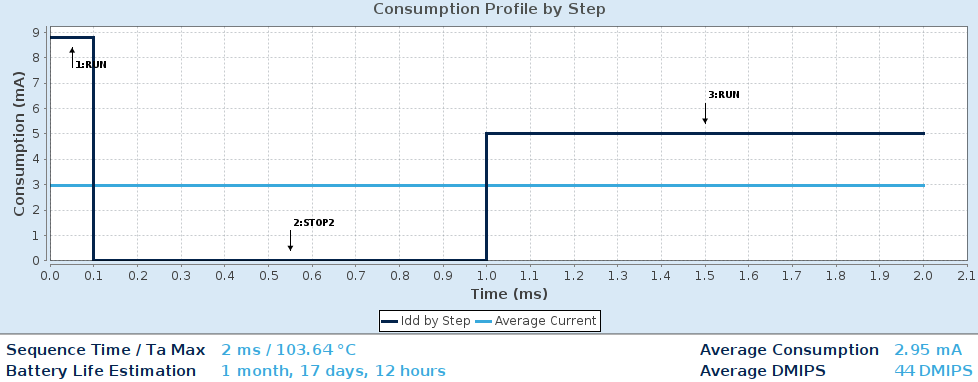
\includegraphics[width=0.99\linewidth]{cube_pcc_advertising_1ms.png} 
	\caption{Symulacja zużycia energii przez urządzenie \gls{BLE} podczas ogłaszania}
	\label{rys:cube_pcc_advertising_1ms}
\end{figure}

Postępując zgodnie z dokumentacją, wykonano dwie symulacje. Rysunek~\ref{rys:cube_pcc_advertising_1ms}
odzwierciedla przewidywane zużycie energii urządzenia BLE dla domyślnie proponowanych nastaw sugerowane przez \textit{PCC}.
Krok trzeci jest etapem aktywacji radia rozgłaszającego komunikaty o~gotowości do połączenia. Szacowany
pobór prądu wynosi ok. 5mA, przy średniej 2.95mA. Jako główne źródło zasilania, do celów
symulacji, dobrano \enquote{\textit{wirtualną}} baterię 3.3V -- Li-SOCL2 (A3400). Umotywowane jest to wykorzystywaniem analogicznego źródła
jak podczas właściwego badania. Oprogramowanie sugeruje, iż bateria zostanie rozładowana po nieco ponad półtora
miesiąca użytkowania.

Analogiczną symulację przeprowadzono dla połączonego już urządzenia -- Rysunek~\ref{rys:cube_pcc_connected_master}.
Dla zadanych parametrów, oczekiwana długość życia układu będzie o~dwie godziny dłuższa niż wcześniej wspomniany
przypadek.

\begin{figure}[!ht]
	\centering 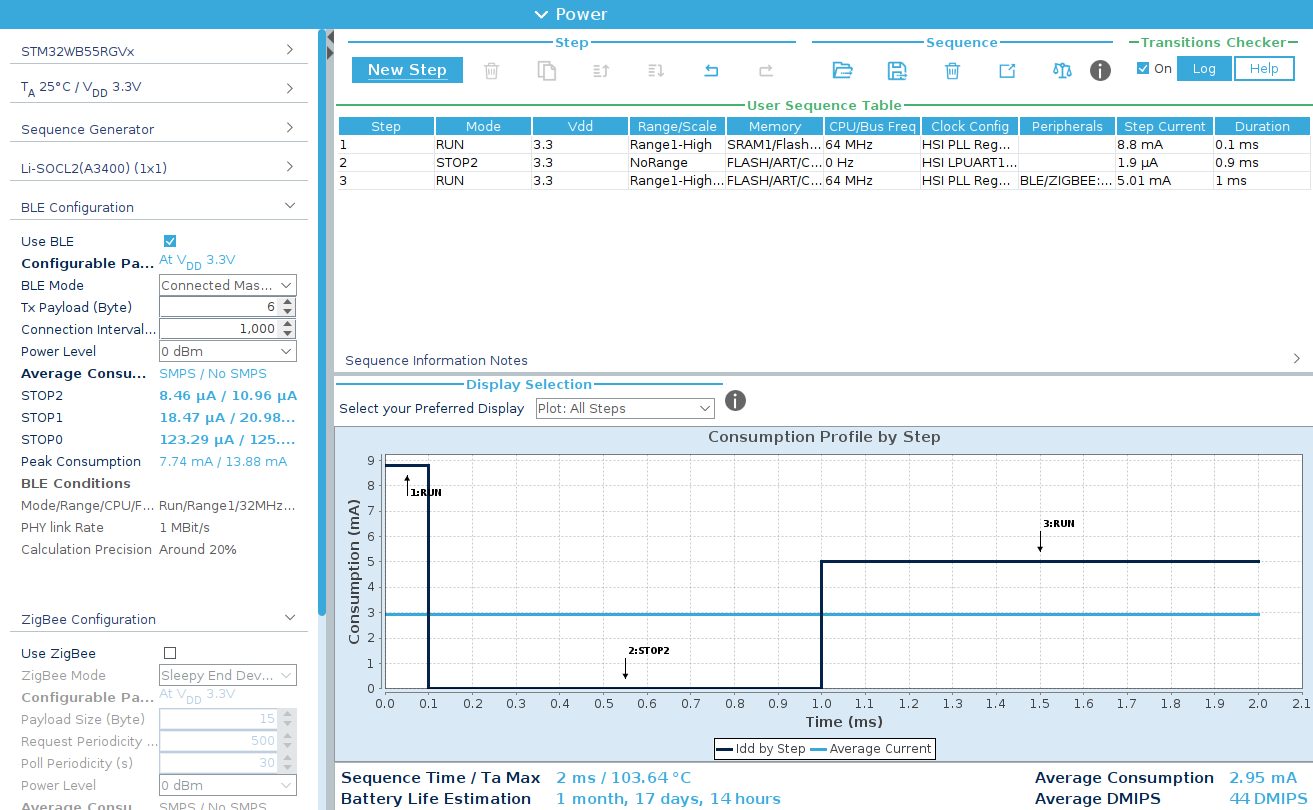
\includegraphics[width=0.99\linewidth]{cube_pcc_connected_master.png} 
	\caption{Symulacja zużycia energii przez urządzenie \gls{BLE} podczas połączenia}
	\label{rys:cube_pcc_connected_master}
\end{figure}

Moduł \textit{PCC} niestety nie zapewnia wsparcia do symulacji węzłów sieci Mesh. Stawia się hipotezę,
iż zużycie energii będzie zależało od poszczególnie pełnionych ról przez dane urządzenie. Standard
przewiduje wykorzystywania zasilania bateryjnego przez węzeł \gls{LPN}. W przypadku takiej konfiguracji,
należałoby spodziewać się rezultatów podobnych do symulowanych. Przeprowadzając pomiary, wykorzystano
standardowe węzły, stale nasłuchujące za sygnałem będąc serwerem modelu \textit{Generic OnOff}. Spodziewane
jest znaczący wzrost zużycia energii właśnie ze względu na wymieniony fakt zaczerpnięty ze specyfikacji.

Zebrawszy dane chwilowych poboru natężenia prądu w czasie, należy wyliczyć właściwe parametry w~postaci
skonsumowanej energii i~mocy. Wykorzystuje się w celu oczywistą zależność fizyczną zaprezentowaną
wzorem~\ref{energy_equation}~\cite{skoro_marta_fizyka_1973}. Wzór uwzględnia okres trwania akwizycji danych
zdefiniowany w~docelowym podrozdziale~\ref{experiment:energy-consumption}.

\begin{equation} \label{energy_equation}
E_{\text{całkowita}} = U \cdot \int_{t=0[s]}^{t=50[s]} \mathrm{d}i \: \mathrm{d} t
\end{equation}

\begin{equation} \label{power_equation}
P = \frac{E_{\text{całkowita}}}{t}
\end{equation}

gdzie:

\begin{description}
\item $E_{\text{całkowita}} [J]$ - wykorzystana energia podczas 50s sekundowej sesji rejestracji danych
\item $P [W]$ - mocz użyta podczas 50s sekundowej sesji rejestracji danych
\item $U [V]$ - napięcie zasilania mikrokontrolera - $3.3V$ - stała
\item $\mathrm{d}i [A]$ - prąd w danej chwili
\item $\mathrm{d}t [s]$ - podstawa czasowa całkowania, 0.01s/interwał ($100Hz$) - stała 
\end{description}

\subsubsection{Badanie Packet Error Rate}\label{subsec:per_experiment}
Przed przystąpieniem do badań należy precyzyjnie zdefiniować wykorzystywaną terminologię.

Pakietem nazywamy pojedynczą porcję danych przetwarzaną na poziomie warstwy sieciowej modelu ISO OSI \cite{sa_tcpip_nodate}.
Warstwa ta umożliwia routing, adresowanie logiczne oraz przetwarzanie i~dostarczanie pakietów.

\begin{figure}[!ht]
	\centering 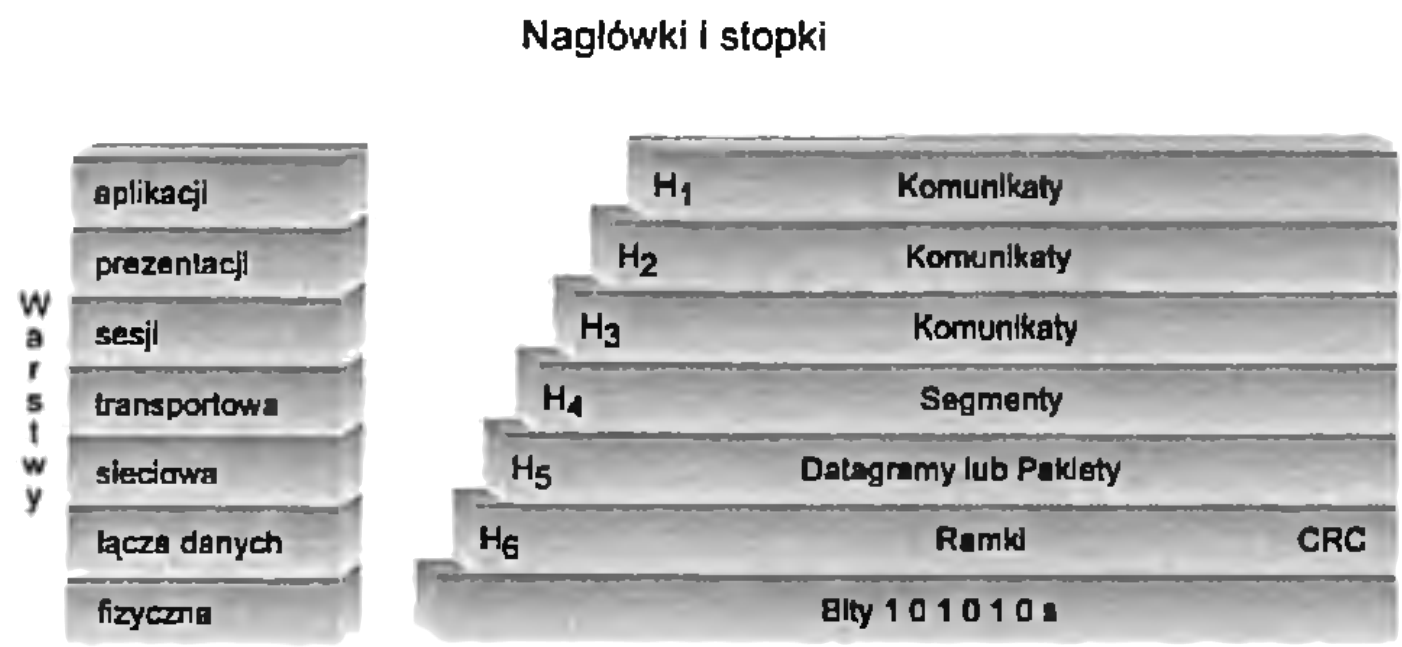
\includegraphics[width=0.618\linewidth]{tcp_ip_szkola_programowania_naglowki_stopki.png} 
	\caption{Model ISO OSI wraz i odpowiadające mu nazwy porcji danych. Źródło: \cite{sa_tcpip_nodate}}
	\label{rys:iso_osi_model_nazwy_grup_danych}
\end{figure}

\gls{BLE} wprowadza własną nomenklaturę dla poszczególnych warstw sieciowych. Jest to o~tyle istotne, iż standard ten
nie zapewnia odpowiadających modelowi ISO OSI warstw jeden-do-jednego. Część z~tych warstw jest agregowanych w~zespół 
protokołów wyższych warstw - Rysunek~\ref{rys:agregacja_protokolow_ble}. %rysunek znajduje się w opisie stosu BT

Bazując na definicji modelu OSI oraz stosie BLE, pakietem można nazwać wiadomości będące możliwie blisko
warstwy \textit{\gls{LL}}. Podobną definicję prezentuje dokumentacja ST:
\enquote{Pakiet to pojedyncza oznaczona wiadomość wysłana przez jedno i~odebrana przez 
co najmniej jedno urządzenie.}\footnote{Tłumaczenie własne}~\cite{stmicroelectronics_pm0271_2021}

BLE Mesh dodatkowo wprowadza własne dodatkowe warstwy komunikacji, jak zostało to opisane w~podrozdziale~\ref{sec:ble}.
Każda z wymienionych warstw jest hermetyzowana za pośrednictwem dostarczanego przez producenta \gls{API}.
Middleware może tym samym zostać zamknięty przed dostępem, skutkując brakiem możliwości 
bezpośredniego nasłuchiwania pakietów w~warstwie \gls{LL}. Uwzględniając powyższe czynniki, \textit{pakietem} dla BLE Mesh nazywana będzie wiadomość najbliższa warstwie \gls{LL}.

Posiadając definicję pakietu, \gls{PER} możliwe staje się zdefiniowanie wzoru, a~zarazem znaczenia
głównego celu badań. PER jest miarą ilości błędnych pakietów w proporcji do wszystkich wysłanych 
pakietów, zgodnie ze zdefiniowanym wzorem~\ref{per_equation}.

\begin{equation}
\label{per_equation}
PER = \frac{s - r}{s} \cdot 100\%
\end{equation}

gdzie:

\begin{description}
\item[s] is ilość wysłanych pakietów
\item[r] is ilość odebranych pakietów
\item[s-r] - ilość niepoprawnych/błędnych pakietów
\end{description}

Eksperyment PER przeprowadzany w warunkach terenowych jest narażony na szereg czynników wpływających
na jakość transmisji. Projektowane doświadczenie starało się zawrzeć przynajmniej część z nich, co
zostało to opisane w podrozdziale~\ref{experiment:per}.

Uznając fakt przeprowadzania badań weryfikujących aspekty komunikacji Bluetooth opartej na częstotliwości
2.4GHz, naturalnym staje się dobór różnych środowisk, w których ten czynnik jest skrajnie różny.
Uzasadnia się to faktem interferencji fal. Warunki zurbanizowane zapewniają bogate tło radiowe,
w~szczególności oparte o częstotliwości będące wykorzystywane przez inne popularne technologie
takie jak WiFi. Zakłada się, iż w takim środowisku prawdopodobieństwo kolizji (interferencji)
jest większe aniżeli w środowisku względnie radiowo odizolowanym. Tym samym, jedną z~badanych
hipotez określa się jako dominujący wpływ tła radiowego w warunkach zurbanizowanych na wzrost
miary \gls{PER}. Analogicznie, w warunkach odizolowanych radiowych, oczekiwany jest mniejsze
tempo wzrostu PER wraz ze zwiększanym dystansem pomiędzy węzłami.

Czynnikiem który może mieć wpływ na rezultaty jest rozmieszczenie węzłów sieci. Zgodnie
z~opisem metodologii (podrozdział~\ref{experiment:per}), każde z urządzeń układane było
bezpośrednio na glebie. Konsekwencją takie stanu rzeczy jest wpływ zjawiska zwanego
rozchodzeniem się fali powierzchniowej. Zgodnie z definicją: \enquote{[antena] jest umieszczona na powierzchni
ziemi, jeśli zawieszono ją na wysokości mniejszej niż $\lambda$ nad powierzchnią}~\cite{szostka_fale_2006}. 
W~przypadku wykorzystania komunikacji Bluetooth, definicję spełnia każde położenie
urządzenia poniżej linii 12,5cm nad powierzchnią ziemi.

Nie mniej istotna na ostateczne efekty badań jest pogoda w postaci czynników temperatury
czy wilgotności. Zmiana w tych parametrach wpływa na wartości tłumienia sygnału.

